\documentclass[onecolumn, draftclsnofoot,10pt, compsoc]{IEEEtran}
\usepackage{graphicx}
\usepackage{url}
\usepackage{float}
\usepackage{setspace}

\usepackage[colorinlistoftodos]{todonotes}%Take out when complete, allows intext comments during work

\usepackage{geometry}
\geometry{textheight=9.5in, textwidth=7in}

% 1. Fill in these details
\def \CapstoneTeamName{		Team Sandy}
\def \CapstoneTeamNumber{		44}
\def \GroupMemberOne{			Raja Petroff			}
\def \GroupMemberTwo{			Andrew Soltesz			}
\def \GroupMemberThree{			Mark Sprouse}
\def \CapstoneProjectName{		AR Sandbox for Construction Planning}
\def \CapstoneSponsorCompany{	Oregon State University}
\def \CapstoneSponsorPerson{		Dr. Joseph Louis}
\title{Design Document}

% 2. Uncomment the appropriate line below so that the document type works
\def \DocType{		%Problem Statement
				%Requirements Document
				%Technology Review
				Design Document
				%Progress Report
				}
			
\newcommand{\NameSigPair}[1]{\par
\makebox[2.75in][r]{#1} \hfil 	\makebox[3.25in]{\makebox[2.25in]{\hrulefill} \hfill		\makebox[.75in]{\hrulefill}}
\par\vspace{-12pt} \textit{\tiny\noindent
\makebox[2.75in]{} \hfil		\makebox[3.25in]{\makebox[2.25in][r]{Signature} \hfill	\makebox[.75in][r]{Date}}}}
% 3. If the document is not to be signed, uncomment the RENEWcommand below
\renewcommand{\NameSigPair}[1]{#1}

%%%%%%%%%%%%%%%%%%%%%%%%%%%%%%%%%%%%%%%
\begin{document}
\begin{titlepage}
    \pagenumbering{gobble}
    \begin{singlespace}
    	%
\includegraphics[height=4cm]{coe_v_spot1}
        \hfill 
        % 4. If you have a logo, use this includegraphics command to put it on the coversheet.
        %\includegraphics[height=4cm]{CompanyLogo}   
        \par\vspace{.2in}
        \centering
        \scshape{
            \huge CS Capstone \DocType \par
            {\large\today}\par
            \vspace{.5in}
            \textbf{\Huge\CapstoneProjectName}\par
            \vfill
            {\large Prepared for}\par
            \Huge \CapstoneSponsorCompany\par
            \vspace{5pt}
            {\Large\NameSigPair{\CapstoneSponsorPerson}\par}
            {\large Prepared by }\par
            Group\CapstoneTeamNumber\par
            % 5. comment out the line below this one if you do not wish to name your team
            %\CapstoneTeamName\par 
            \vspace{5pt}
            {\Large
                \NameSigPair{\GroupMemberOne}\par
                \NameSigPair{\GroupMemberTwo}\par
                \NameSigPair{\GroupMemberThree}\par
            }
            \vspace{20pt}
        }
        \begin{abstract}
        % 6. Fill in your abstract    
      	The purpose of this document is to describe how we plan on implementing the required functionality of the AR Sandbox.
        This means describing how the various display modes, such as calibration, depth, design, and cut and fill, will work, as well as the lower level graphics systems that are necessary for these display modes to function.
        Finally, we discuss the data generated and stored by the software, as well as the actual physical components of the AR Sandbox itself.
        \end{abstract}     
    \end{singlespace}
\end{titlepage}
\newpage
\pagenumbering{arabic}
\tableofcontents
% 7. uncomment this (if applicable). Consider adding a page break.
\listoffigures
%\listoftables
\clearpage

% 8. now you write!
\section{Introduction}

\subsection{Purpose}
This document describes the design and architecture for the AR Sandbox. Based on the requirements set in the corresponding Software Requirements Document, the design document elaborates on how the system is made.

\subsection{Scope}
This document expands on the features defined in the Software Requirements Document, by describing the implementation and data flow required to achieve the desired functionality. This document will cover the development timeline, testing protocols, and the API of the system.

%\subsection{References}
%Original UC Davis AR Sandbox: https://arsandbox.ucdavis.edu/

\subsection{Glossary}
\begin{itemize}
\item Augmented Reality Sandbox (AR Sandbox): A physical sandbox with a depth sensor and projector that displays graphics on the sand, such as roadways and ground topology.
\item Augmented Reality: A term referring to any technology that superimposes computer generated imagery on the real world. In this case, the term refers to the graphics projected onto the sand. When a user manipulates the sand, the graphics displayed on the sand will change.
\item Projection: The image cast on the sand's surface by the projector
\item Depth Sensor: A digital imaging device which uses a grayscale image to represent the distance from the sensor to the nearest surface.
\item SSD: Software Specification Document
\end{itemize}

\section{System Overview}
%Overview of the project as a whole
%Gives a sense for what the entire project will look like
%Higher level

%---------------------------------------------
% Put in intro paragraph.  Mention what 
% they are looking at with the modes section and such
%---------------------------------------------

The AR Sandbox for Construction Planning is an augmented reality sandbox with additional functionality built in for civil engineering applications.
At any point, the sandbox will be set to one of four different modes.
These modes and how they behave are outlined in this section, after the system components are discussed.

\vfill

\subsection{System Components}
\par Figure 1 shows the different hardware and software components of the AR sandbox and how they interact. This diagram serves as a general overview of the entire system, with each component being explored in greater detail later in the document.

\begin{figure}[H] 
	\centering
	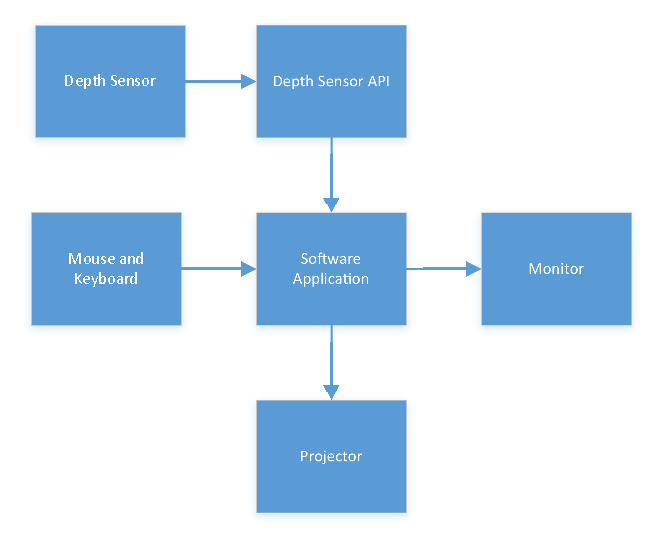
\includegraphics[width=6in]{BlockDiagram}
    \caption{An overview of the system's components and how they interact}
    \label{fig:overview}
\end{figure}

%-----------------------------------------------
% Maybe have more higher level paragraphs explaining the modes and what they do
% As opposed to the low-level list of stimuli and reactions
%-----------------------------------------------

\subsection{System Modes}
\subsubsection{Calibration Mode}
Calibration mode is used to calibrate the depth sensor and projector, mainly for use during the initial set\-up process for the sandbox. A summary of features is listed below:

\begin{itemize}
\item \textbf{User switches to Calibration Mode}
Current bounds of the projection area are shown on the sand.

\item \textbf{User uses the computer terminal to adjust bounds of projection area}
A bounding box appears when the mouse is moved, this box dictates the area defined as the sandbox.

\item \textbf{User calibrates depth sensor by placing an object with flat sides on the sand}
Using height sensor data, the outline of the object is projected onto the sand. 
The computer terminal is used to move this outline around until it lines up with the physical object.

\item \textbf{User changes the current display mode}
The current display information shall be replaced with the information that corresponds to the display mode selected.
\end{itemize}

\subsubsection{Depth Mode}
While in Depth Mode, the program will visually represent the height of the sand using color and contour lines. Below is an overview of Depth Mode's features:

\begin{itemize}
\item \textbf{User observes sandbox}
The different heights at different points along the surface of the sand shall be visually represented via a projection.  This projection will consist of a 2-dimensional representation of the height projected onto the 3-dimensional surface of the sand.

\item \textbf{User physically manipulates the sand, changing the landscape in the box}
The visual representation projected on the sand shall adjust in accordance to the new height of the sand in the areas that have been altered. 

\end{itemize}

\subsubsection{Design Mode}
Design mode is used to control the shape of the road segment that is projected onto the terrain. A summary of features is listed below:

\begin{itemize}
\item \textbf{User switches to Design Mode}
A segment of road is displayed.

\item \textbf{User uses the computer terminal to edit the path of the road}
The user shall be able to adjust the position and curvature of the road.
The user shall be able to place additional manipulation points along the road which can be used to further refine the path of the road.
A edit/reset button shall be present to revert the road back to its previous path.
The User shall be able to undo unwanted changes.

\end{itemize}

\subsubsection{Cut \& Fill Mode}
Cut and Fill mode is used to visualize the volumes of material that must be added or removed in order to achieve the desired road path. A summary of this mode's features is outlined below:

\begin{itemize}
\item \textbf{User observes sandbox}
A road shall be displayed traversing the surface of the sand.  Along this road, the amount of sand that would be required to be taken away or put in place in order to achieve the desired alignments along the road shall be visually represented.  In addition, the total haul quantity, average haul distance, average haul grade, estimated haul duration, and the construction equipment to use shall be displayed.

\item \textbf{User physically manipulates the sand, changing the landscape in the box}
The representation along the road and the additional information described above shall adjust in accordance to the new height of the sand.

\end{itemize}
%---------------------------------
% May want to reorganize these sections.  Just need to cover all bases, how we organize is up to us.
%Also, this is a rough draft, so no matter if we miss a few things.
%---------------------------------
\section{System Architecture}
%Provide a model for our solution
%What is going to make up the system described above?
The purpose of this section is to provide the model of our AR Sandbox System.  
The Architectural Design subsection demonstrates how this system is comprised of various components which interact with one another; these relationships and interactions are explained and displayed with diagrams and figures. 
The Decomposition Description subsection goes into further detail about each of these components and how they are implemented.
Lastly, the Design Rationale subsection provides reasoning behind some of the design choices presented previously.

\subsection{Architectural Design}
\par Figure 2 gives an overview of the software architecture and shows how the different components, such as the heightmap and vertex/fragment shader takes the input from the depth sensor and renders it into a terrain mesh.



\begin{figure}[H]
	\centering
	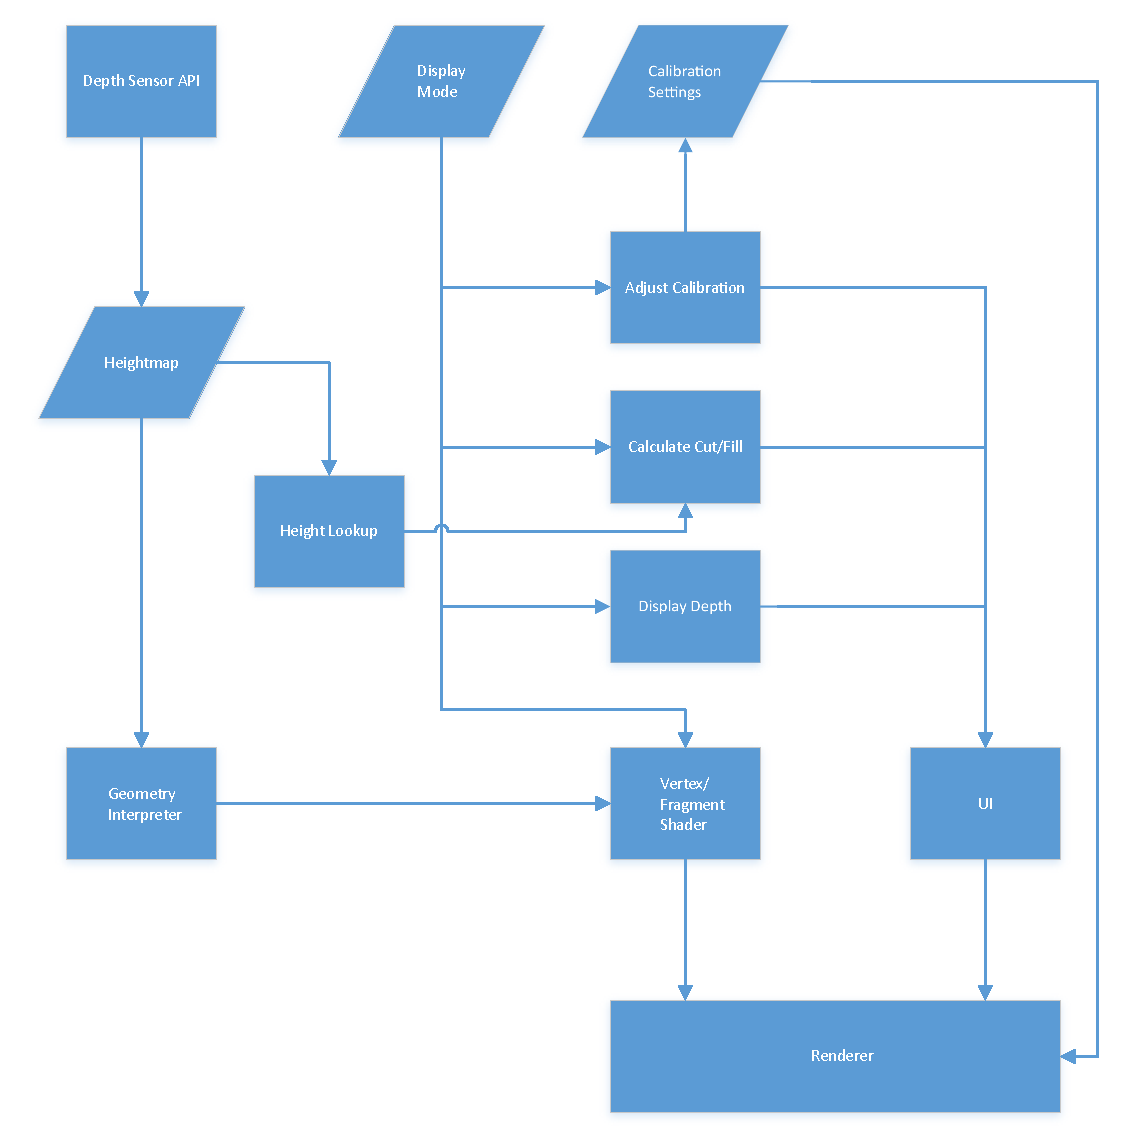
\includegraphics[width=6in]{SysArch}
    \label{fig:sysarchitecture}
\end{figure}

\begin{figure}[H]
	\centering
	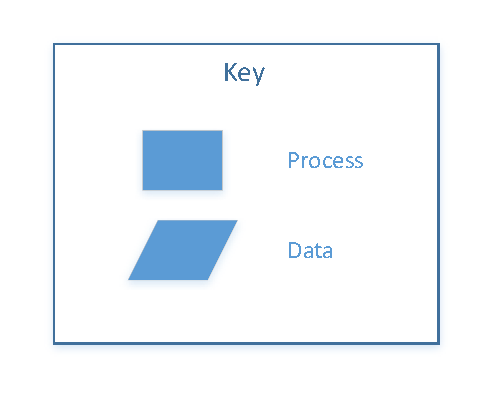
\includegraphics[width=2in]{SysArchKey}
    \caption{System Architecture}
\end{figure}

%\subsection{Decomposition Description}
%Talk about the nodes described in Arch. Design. 
\subsubsection{Depth Sensor API} %Mark

The Kinect's API allows for the Kinect sensor to interface with the rest of the sandbox system.
It provides access to the sensor's depth image data, raw infrared image, full-color image, and has built-in body tracking functionality \cite{kinect_api_overview}.
For this system, the API's primary functionality will be providing the sensor's depth image data which will be stored as the heightmap.


\subsubsection{Geometry Interpreter} %Andrew
The Geometry Interpreter takes the heightmap data from the depth sensor and converts it into a three dimensional mesh.
It is responsible for performing any downsampling required to make the mesh renderable in real time.

\subsubsection{Height Lookup}
The height lookup module is responsible for fulfilling requests for height data at a given point on the terrain mesh.
This is accomplished by correlating the point in 3-space to a pixel on the heightmap, and multiplying the resulting greyscale (normalized to 1) value by the maximum height of the terrain.

\subsubsection{Adjust Calibration} %Mark
Adjust Calibration is used to adjust system settings in order to ensure the sensor and projector are properly aligned with each other as well as the surface of the sand.  
These setting include adjustments in area the depth sensor is looking in and the area covered by the projection.
This module continually interacts with the UI as it prompts the user with the setting to be adjusted and then stores these settings in the Calibration Settings.

\subsubsection{Calculate Cut/Fill} %Raja
Cut and fill refers to the process of creating a level path where a road or highway can be built.
The cut or fill of a road will be calculated by determining the height of a part of the sand where the road should be, then displaying a colored view of the road.
For example, if the road is below a certain height, the it's displayed using a shade of blue.
If it's above a certain height, the road is displayed using a shade of red.

\subsubsection{Display Depth} %Raja
Display depth is used to visualize the height or altitude of an area.
If a part of the sand is above a certain height, then it's displayed using a shade of red.
If the sand is below a certain height, then is displayed using a shade of blue.
The intensity of the color depends on how far the height of the sand is from a predetermined height.

\subsubsection{Vertex/Fragment Shader} %Andrew
This program utilizes two pairs of vertex and fragment shaders written in the OpenGL Shader Language (GLSL). 
The first is responsible for coloring the terrain mesh in order to visually represent height information. 
The second is used to color road segments to represent cut and fill data. 
The visual appearance of these shaders will change depending on the current display mode.

\subsubsection{User Interface} %Raja
The user interface allows the user to manipulate the design of the road or change the display mode.
The user will interface with the software via a standard computer terminal with a mouse and keyboard.
The user can also manipulate the sand which will change the topography outputted by the software.

\subsubsection{Renderer}  %Andrew
The rendering subsystem is handled by the Unity engine, and is accessed indirectly through shaders and Unity's UI system.

\subsection{Design Rationale}
%Why did we choose this design choice?
Since the software is being built using the Unity Engine, some of our design choices such as the discrete UI subsystem and choice of shader language are limited to what Unity supports. Use of a bitmap image to represent height is determined by the output of the depth sensor. 
The decision to separate different display modes into distinct modules allows for extensibility should another developer wish to add additional modes.

\section{Physical Architecture} %Mark
%Provide a model for our solution
%What is going to make up the system described above?


\subsection{Architectural Design}
Figure 3 shows the physical design of our AR sandbox.
The sandbox is a mobile box filled with sand and has an arm with a projector and depth sensor connected to an adjacent computer terminal. The components related to the physical architecture of the sandbox are described below.

\begin{figure}[H]
	\centering
	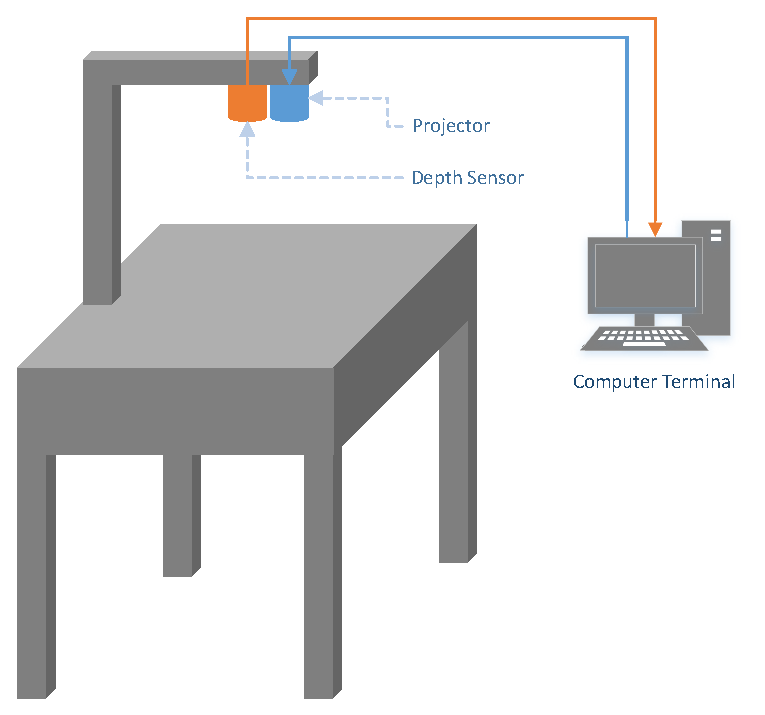
\includegraphics[width=6in]{PhysicalDiagram}
    \caption{Physical Architecture}
    \label{fig:physicalarchitecture}
\end{figure}

\subsubsection{Depth Sensor}

The depth sensor that will be used is a Kinect Sensor by Microsoft.  
The Kinect comes equipped with a 1280x960 full-color camera, and a Infra-Red light emitter and sensor along with an array of microphones and a tilt motor.
For this project's purposes, the Kinect's IR sensor and emitter will be primarily used and will allow us to capture a depth image.
This Infra-Red system offers a workable range of 0.8m to 3.5m from the target with a data precision of 1cm \cite{andersen_jensen_lisouski_2012}.

\subsubsection{Projector}

The Projector that will be used is a AAXA M5 Mini Portable Business Projector.
This 6in X 6in X 1.8in box only weighs 1.9 pounds and offers a 1280x800p picture at 900 lumens.
Allowing for a screen up to 150in, this projector allows for a very bright and clear image for its size.


\subsubsection{Computer Terminal}
To power the AR sandbox, we will be using an HP Z240 full tower desktop computer with 16 GB of RAM, a 1TB spinning disk, and an Intel core i7 processor with a base speed of 4.2 GHz. We will install an Nvidia GTX 10XX series graphics card to handle rendering.

\subsection{Design Rationale}
%Why did we choose this design choice?

When choosing the Kinect, the most important factors were the accuracy the sensor and its API.
The Kinect is one of the most accurate depth sensors on the common market and the API created by Microsoft has been created specifically for developers to use when utilizing the sensor for their applications.

The most important factors of the projector are its size/weight and its brightness.
Because of the way the projector is going to be mounted above the box, a smaller and light projector was necessary for proper stability.
With the majority of projectors at this size providing a brightness of 50-100 lumens, the 900 lumens is phenomenal.

In regards to the computer terminal, it is necessary to use a full tower desktop since a majority of graphics cards are too big to fit in a small form factor machine, or lack the hardware to mount in such a computer. Using an Nvidia GTX graphics card will give us the best results for rendering real time graphics at the lowest cost when compared to a similar workstation graphics card.

\section{Data Design} %Andrew
%How is the data going to flow?
%How is it stored?
This section discusses the specifications for the data that will be utilized by the system. The data types and methods for data storage are covered.
\subsection{Data Description}
The main piece of data utilized by this system is the height data received by the depth sensor API. This data is represented both as a three dimensional mesh and as a greyscale bitmap image. 
This is because the mesh must be downsampled in order to render efficiently, which, if it were the sole source of height data, would decrease the accuracy of any calculations. 
The benefit of coupling the mesh to a heightmap is twofold: first, the original data accuracy is maintained, while still reaping the benefits of improved rendering, and secondly, obtaining the height at a specific point can be made much faster since this information can be obtained through a simple texture lookup rather than through mathematical calculation.  

\subsection{Data Dictionary}
\subsubsection{Heightmap}
The heightmap is a greyscale bitmap image, in which each pixel represents a relative height. 
Each pixel is represented with 8 bits, yielding 256 shades of grey. 
In order to correlate a pixel to a y-value in 3-space, its value must be multiplied by a constant maximum terrain height. 
This is because the heightmap represents the \textit{average} height, where the lowest point is represented by a value of 0, and the highest point is represented by a value of 256.
\subsubsection{Terrain Mesh}
The terrain mesh is generated by the geometry interpreter, which converts the heightmap into a three dimensional mesh. This mesh is what is rendered by the game engine and what is colored by the shader.
%maybe do a subsubsection on the "application context" IE: the program's state/global vars

% \section{Human Interface Design} %Raja
% \subsection{Architecture Design}
% \begin{figure}[H]
% 	\centering
% 	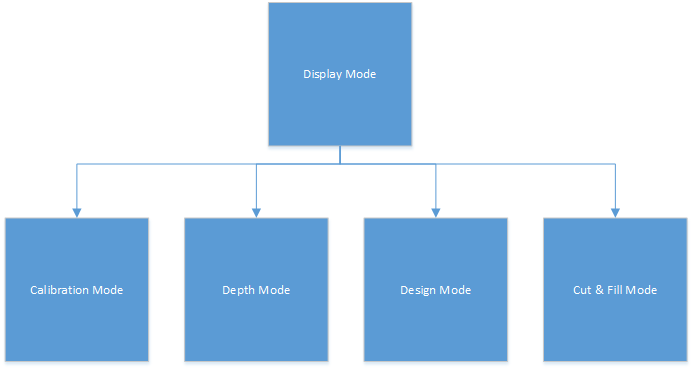
\includegraphics[width=6in]{UI}
%     \caption{User Interface Architecture}
%     \label{fig:uiarchitecture}
% \end{figure}

% \subsection{Decomposition Description}
% \subsubsection{Display Mode}

% \subsection{Design Rationale}
% The user interface is a way for the user to change the mode of operation, as well as manipulate certain aspects such as the layout of the road.

\pagebreak
\bibliographystyle{IEEEtran}
\bibliography{references}

%\appendix

\end{document}